\chapter{Unsigned Multiplication}

Algorithm 1
\begin{enumerate}
    \item set \emph{v} to 0
    \item for each digit do:
    \begin{enumerate}
        \item if lsb of \emph{x} is 1, add \emph{y} to \emph{v}
        \item left shift \emph{y}
        \item right shift \emph{x}
    \end{enumerate}
\end{enumerate}

This basically only handles numbers whose product fits in 1 register.  In general multiplication could take up to 2 registers.

\noindent
Algorithm 2
\begin{enumerate}
    \item group two regs (\emph{u},\emph{v}) for product, set to 0
    \item for each digit do:
    \begin{enumerate}
        \item  add (\emph{y} and lsb(x)) to \emph{u} hold carry in \emph{c}
        \item right shift (\emph{c},\emph{u},\emph{v})
        \item circulant right shift \emph{x}
    \end{enumerate}
\end{enumerate}

Right shifting the product with carry is the same as left shifting (\emph{$y_{hi}$},\emph{y}), but without the need for a second register to hold the high order bits.  The algorithm can be implemented in a circuit as is done in Figure~\ref{f-unsigned_mult}.

\begin{figure}
\caption{Unsigned Multiplier of Algorithm 2}\label{f-unsigned_mult}
\begin{center}
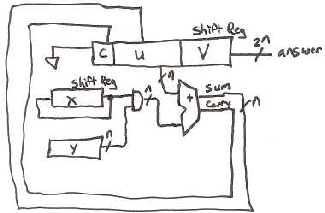
\includegraphics{unsigned_mult.png}
\end{center}
\end{figure}

\begin{example}
Multiply 10 and 12 in binary using algorithm 2

{\color{ans}
First we need to convert our numbers to binary: $x=10_{10} = 1010_2$ and $y=12_{10} = 1100_2$.

\begin{tabular}{ccccp{2in}}
c & u    & v    & x    & Comments  \\\hline
0 & 0000 & 0000 & 1010 & Setup (Step 1) \\\hline
  &      &      &      & Round 1\\
0 & 0000 &      &      & Step 2a: add $y\cdot 0$ to u (0+0=0)\\
0 & 0000 & 0000 &      & Step 2b: rotate right cuv \\
  &      &      & 0101 & Step 2c: circulant right shift x \\
0 & 0000 & 0000 & 0101 & End of round 1 \\\hline
  &      &      &      & Round 2\\
0 & 1100 &      &      & Step 2a: add $y\cdot 1$ to u (0+12=12)\\
0 & 0110 & 0000 &      & Step 2b: rotate right cuv \\
  &      &      & 1010 & Step 2c: circulant right shift x \\
0 & 0110 & 0000 & 1010 & End of round 2 \\\hline
  &      &      &      & Round 3\\
0 & 0110 &      &      & Step 2a: add $y\cdot 0$ to u (6+0=6)\\
0 & 0011 & 0000 &      & Step 2b: rotate right cuv \\
  &      &      & 0101 & Step 2c: circulant right shift x \\
0 & 0011 & 0000 & 0101 & End of round 3 \\\hline
  &      &      &      & Round 4\\
0 & 1111 &      &      & Step 2a: add $y\cdot 1$ to u (3+12=15)\\
0 & 0111 & 1000 &      & Step 2b: rotate right cuv \\
  &      &      & 1010 & Step 2c: circulant right shift x \\
0 & 0111 & 1000 & 1010 & End of round 4 \\\hline
\end{tabular}

Note $x$ is returned to its original value and $uv = 01111000_2 = 120_{10}$.
}
\end{example}

\begin{example}
Multiply 14 and 7 in binary using algorithm 2

{\color{ans}
First we need to convert our numbers to binary: $x=14_{10} = 1110_2$ and $y=7_{10} = 0111_2$.

\begin{tabular}{ccccp{2in}}
c & u    & v    & x    & Comments  \\\hline
0 & 0000 & 0000 & 1110 & Setup (Step 1) \\\hline
  &      &      &      & Round 1\\
0 & 0000 &      &      & Step 2a: add $y\cdot 0$ to u (0+0=0) \\
0 & 0000 & 0000 &      & Step 2b: rotate right cuv \\
  &      &      & 0111 & Step 2c: circulant right shift x \\
0 & 0000 & 0000 & 0111 & End of round 1 \\\hline
  &      &      &      & Round 2\\
0 & 0111 &      &      & Step 2a: add $y\cdot 1$ to u (0+7=7) \\
0 & 0011 & 1000 &      & Step 2b: rotate right cuv \\
  &      &      & 1011 & Step 2c: circulant right shift x \\
0 & 0011 & 1000 & 1011 & End of round 2 \\\hline
  &      &      &      & Round 3\\
0 & 1010 &      &      & Step 2a: add $y\cdot 1$ to u (3+7=10) \\
0 & 0101 & 0100 &      & Step 2b: rotate right cuv \\
  &      &      & 1101 & Step 2c: circulant right shift x \\
0 & 0101 & 0100 & 1101 & End of round 3 \\\hline
  &      &      &      & Round 4\\
0 & 1100 &      &      & Step 2a: add $y\cdot 1$ to u (5+7=12) \\
0 & 0110 & 0010 &      & Step 2b: rotate right cuv \\
  &      &      & 1110 & Step 2c: circulant right shift x \\
0 & 0110 & 0010 & 1110 & End of round 4 \\\hline
\end{tabular}

Note $x$ is returned to its original value and $uv = 01100100_2 = 98_{10}$.
}
\end{example}

